\section{Objetivos y contextualización}

  Actualmente, la empresa tiene más de 700 clientes activos, cada uno con diferentes contratos, o condiciones comerciales, y se utiliza un archivo de Excel para mantener estas condiciones actualizadas. Al mismo tiempo, este excel también contiene la forma en que se calculan los costos totales por el uso del servicio para cada cliente. Similar a lo que ocurría con la falta de pruebas automatizadas, también resulta curioso el hecho de que Beetrack, siendo una empresa SaaS y teniendo su propio ERP, utilice esta plantilla para calcular cuánto cobrarle a los clientes. Es por lo anterior que decidió crear un servicio especializado en el almacenamiento y cálculo de estas condiciones comerciales, y cuyo único propósito fuese resolver el problema de cómo calcular los costos por cliente y poder almacenar los modelos que representaran los contratos generados con estos.
  
  Uno de los puntos más cruciales sobre este servicio y su contexto es el hecho de que ya se había intentado dos veces algo similar. El primer intento fue mediante un desarrollo interno en el ERP, el cual no tuvo los resultados esperados en términos de precisión al momento de facturar y se concluyó que no era responsabilidad de \textit{Hive} como tal tener esta información. El segundo intento fue la migración de estos planes a un proyecto que, en su minuto, se encontraba en fase \textit{beta} en Hubspot, en el cual se prometía poder tener la información siempre actualizada. Finalmente terminó ocurriendo lo mismo que en el primer intento, pero con peor precisión al momento de facturar de manera automática, entregando, en el mejor de los casos, una precisión de 43\%.

  Teniendo en consideración los requisitos y los resultados anteriores, los objetivos principales del proyecto fueron dos. El primer objetivo, fue construir un modelo lo suficientemente flexible como para poder abarcar los diferentes tipos de ventas que los vendedores realizan, tanto para productos como servicios. El segundo objetivo fue el programar un servicio de resolución comercial, o calculadora, que fuese, nuevamente, lo suficientemente flexible como para poder abarcar el modelo, pero que al mismo tiempo no necesitara información contextual más allá del uso para saber cuánto cobrarle a cada cliente, mientras que al mismo tiempo entregaba glosas prehechas por producto.

  El equipo de Operaciones decidió no acoplar este proyecto a \textit{Hive} de manera de evitar el cruce indebido de información y para así poder mantener las ideas aisladas y para así comenzar a tener una arquitectura de sistemas distribuidos en base a servicios. Lo anterior sumado al hecho de que el se prevee que, eventualmente, otros servicios y productos de la empresan, tales como el \textit{Customer Portal}, consuman los recursos expuestos por este servicio de manera de que los clientes también puedan saber cuánto se les cobrará o el nivel de costo que tienen para un día determinado del mes. Como se puede ver en la figura \ref{fig:arquitectura}, del capítulo \ref{metodologias}, la arquitectura que se decidió utilizar es una en la cual el servicio de condiciones está aislada del ERP, mientras que al mismo tiempo no limita a que otro servicio pueda consumir la información del servicio nuevo, lo cual hubiese ocurrido en caso de haber escrito el código en \textit{Hive} dada su naturaleza monolítica.

\section{Desarrollo}

  \subsection{Modelamiento}

    El proceso de desarrollo del nuevo servicio de condiciones comerciales comenzó con un análisis de los diferentes planes existentes y que se encuentraban en uso en por parte de la empresa. Luego de realizar este análisis se definieron 4 modelos diferentes a nivel de base de datos que permitirían almacenar de manera flexible las condiciones con las cuales se les factura a los clientes. 
    
    En primer lugar se tiene el modelo del plan, en este se almacena la condición comercial como tal, junto con una descripción del uso que puede tener esta condición y el producto y moneda asociado a la condición. Dentro del campo ``\texttt{condition}'' se almacena el tipo de tramo y costos asociado que tendrá por ellos. Se decidió que se puede tener tres tipos de tramos diferentes: base, variable y por paso. A continuación se detalla cada tipo de tramo:
    \begin{enumerate}
      \item Tramo base: va desde cero unidades hasta la cantidad de unidades determinada con un costo fijo total por esas unidades. Solamente se puede tener un tramo de este tipo por plan.
      \item Tramo variable: funcionan mediante una definición de inicio a final del tramo en término de cantidad de unidades, con un precio unitario por la cantidad de unidades utilizadas. Se pueden tener entyre cero e infinitos tramos variables por plan.
      \item Tramo por pasos: se utilizan para poder representar los productos que se venden mediante paquetes, esto es especialmente útil para el servicio de correos en el cual se cobra mediante paquetes de 10.000 correos, siendo los primeros 10.000 gratis y los siguientes teniendo un costo de 1 UF por bolsa adicional. Este tipo de tramo es excluyente con los dos anteriores y solo se puede tener, el cual funciona de manera recurrente.
    \end{enumerate}
    
    Adicionalmente, el campo ``\texttt{condition}'' contiene dos variables utilizadas al momento de calcular el costo total al momento de generar la factura para un cliente. Estos se detallan a continuación:
    \begin{enumerate}
      \item \texttt{general\_minimum}: se utiliza para asegurar un monto mínimo de facturación del producto independiente del uso del cliente una vez que ya se haya calculado el costo por el uso que el cliente le haya dado al producto o servicio.
      \item \texttt{add\_base\_to\_variable}: se utiliza al momento de calcular el costo del uso del producto, y sirve para saber si el plan que se negoció con el cliente se entiende de manera de que se cobre sumando el costo base o utilizando el costo unitario del tramo variable en caso de aplicar.
    \end{enumerate}
    
    El esquema de información del campo ``\texttt{condition}'' se puede ver en la figura \ref{fig:cc_condition_schema}, mientras que en la figura \ref{fig:cc_pricing_chart} se puede observar una manera visual de entender el modelo de precios y condiciones comerciales de los clientes.
    
    \begin{figure}
      \centering
      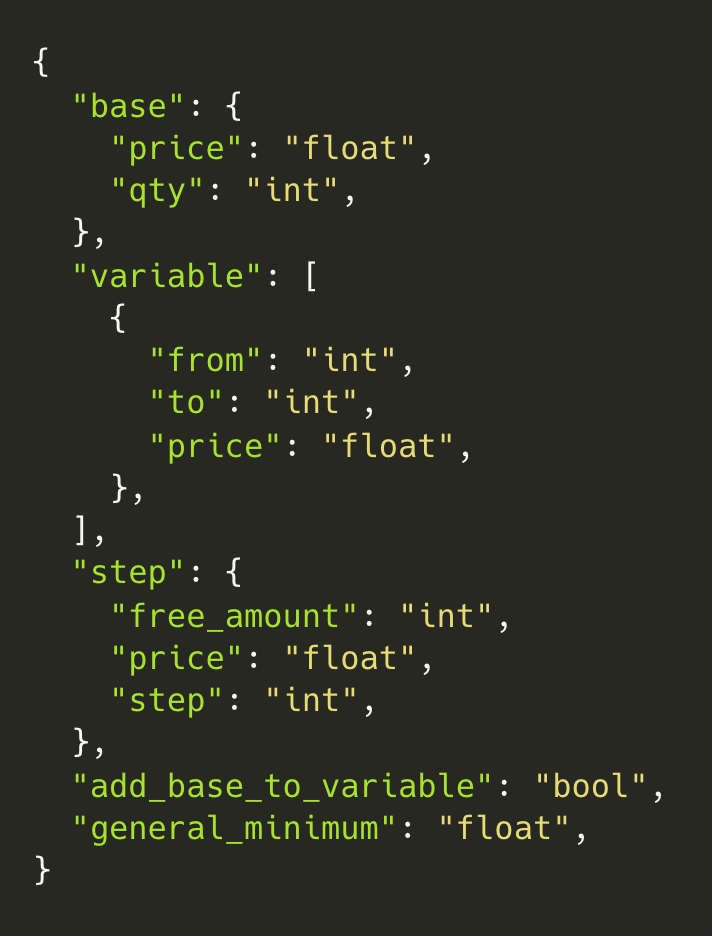
\includegraphics[width=0.4\linewidth]{figures/cc/cc_condition_schema.png}
      \caption{Esquema de información de condición comercial.}
      \label{fig:cc_condition_schema}
    \end{figure}

    \begin{figure}
      \centering
      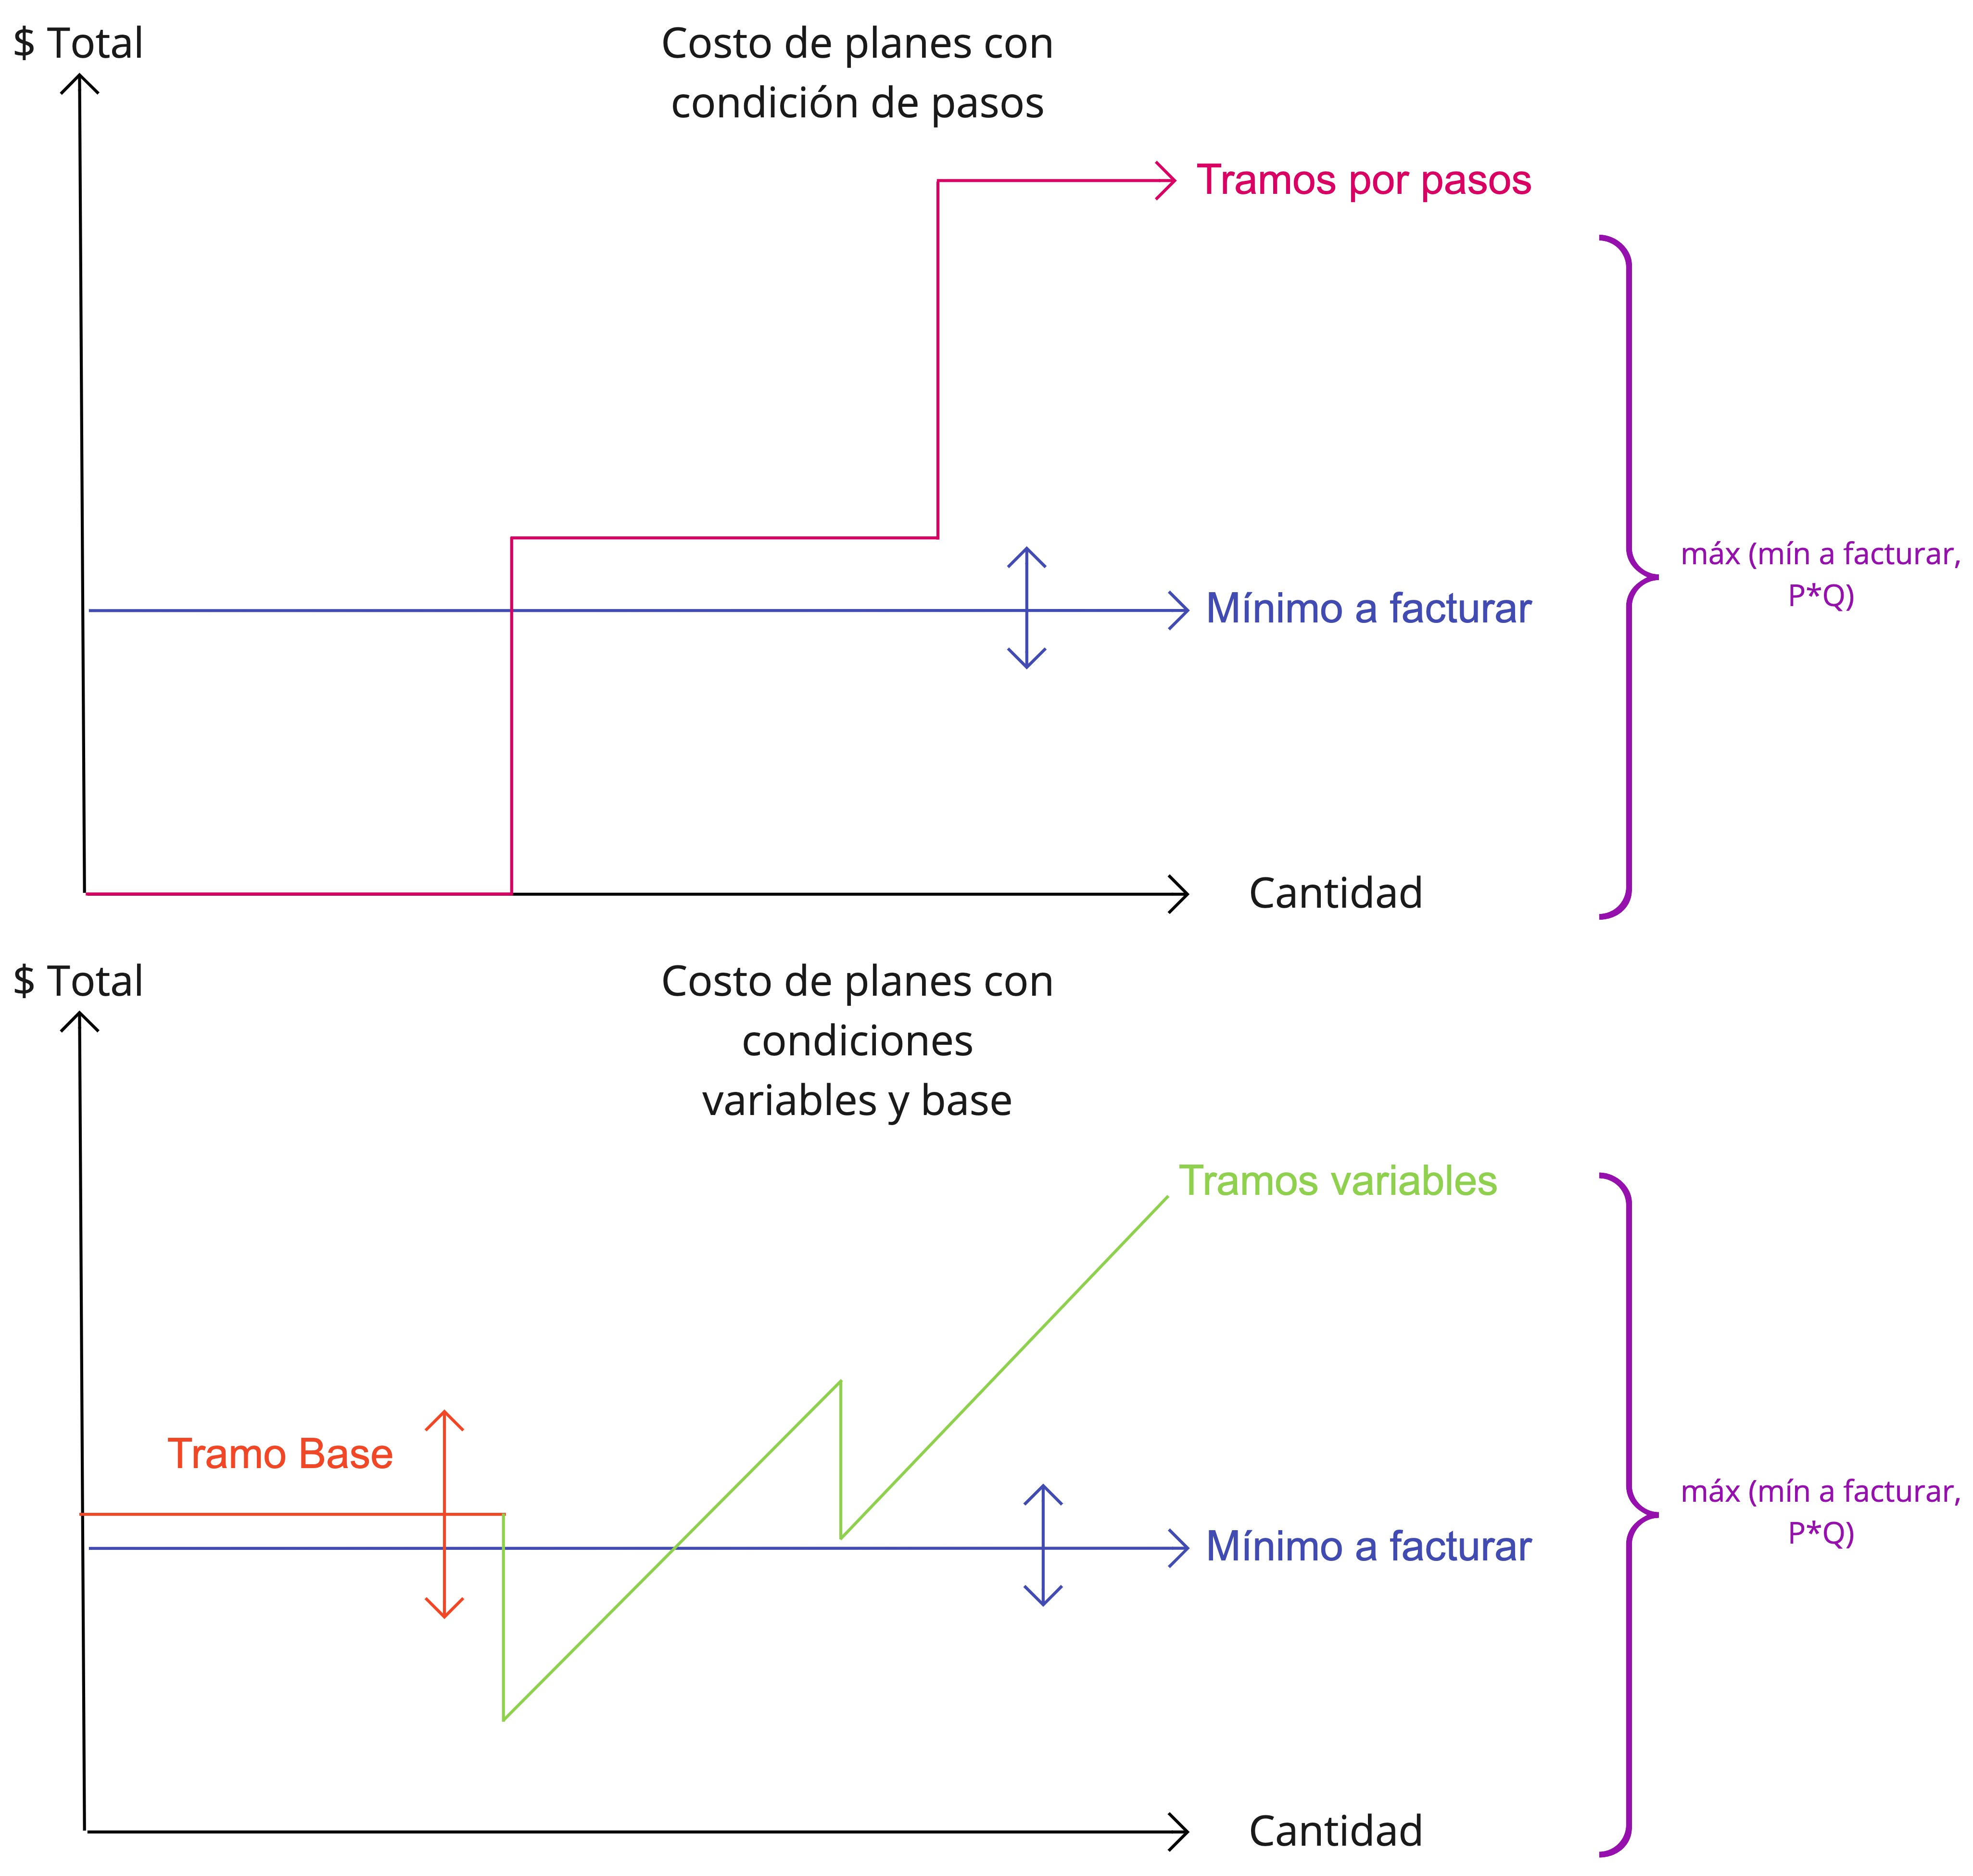
\includegraphics[width=0.6\linewidth]{figures/cc/cc_pricing_chart.jpg}
      \caption{Modelos de cobros y condiciones comerciales.}
      \label{fig:cc_pricing_chart}
    \end{figure}

    En segundo lugar, el modelo de relación plan (\texttt{plan\_relations}) tiene el rol de asociar el contrato del cliente con el plan creado de manera desacoplada y permitiendo la reutilización de planes estándares. 
    
    En tercer lugar, ``\texttt{plan\_relation\_proposals}'' tiene el propósito de permitir que se pueda tener una agrupación de relaciones de planes en un mismo modelo en caso de que un vendedor haya pactado con un cliente condiciones no estándar. Las condiciones estándar se definieron en conjunto con los vendedores a lo largo de múltiples reuiones y una posterior validación de Felipe Porter, jefe del área de ventas de la empresa. En caso de que las condiciones que un vendedor no sean las predefinidas y acordadas se definió que estas requerirían aprobación de Felipe Porter o Sebastián Ojeda (CEO). En caso contrario, las condiciones para el cliente determinado se aprueban de manera automática y se pueden utilizar al momento de facturar.
    
    En cuarto y último lugar el modelo ``\texttt{comments}'', tiene el propósito de simplemente contener el cuerpo del comentario por parte del vendedor en caso de que quiera hacer notar algo de los planes que está creando.

    En la figura \ref{fig:cc_relations} se puede observar los diferentes modelos y sus relaciones, junto con sus campos y tipos de datos por campo.
    
    \begin{figure}
      \centering
      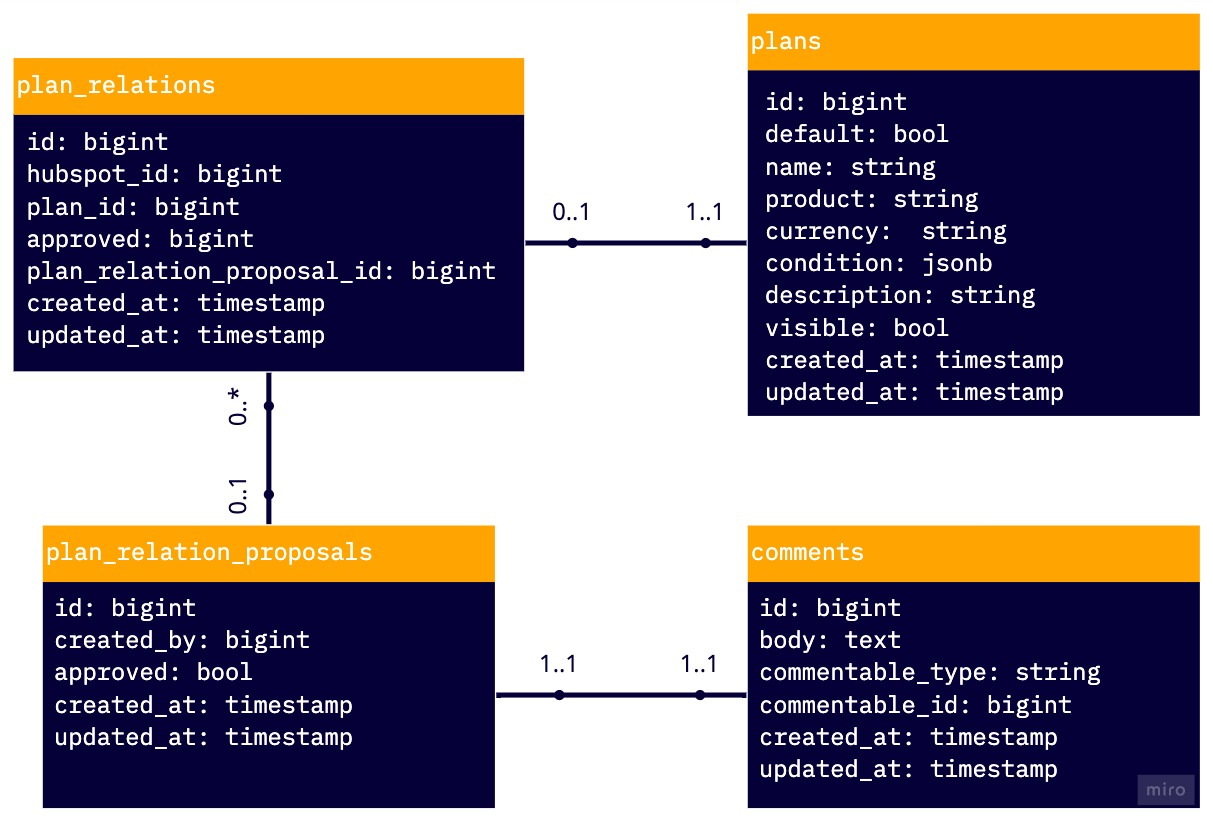
\includegraphics[width=0.75\linewidth]{figures/cc/cc_relations.jpg}
      \caption{Relaciones de modelos de condiciones comerciales.}
      \label{fig:cc_relations}
    \end{figure}
\section{Resultados}